
\subsection{Long-context Safety Mitigation Details} \label{app:lc_safety_mitigation}

\textbf{Supervised finetuning datasets.}
To mitigate many-shot jailbreaking risks (MSJ), we train our long-context models to respond in a safe manner, even when presented with demonstrations of unsafe behavior in context. We construct SFT datasets comprising $k$-shot examples, formatted as multi-turn dialogues, as follows:: 1 example = [ $k$ demonstrations | target query | target response ].

We extract target queries and responses from adversarial and borderline SFT datasets, maintaining a 1:2 ratio between the two. We create demonstration pairs (<prompt, response>) by following the protocol of \cite{anil2024many}, with both benign/borderline (B) and harmful (H) content, resulting in the following combinations: BB, BH, HB, HH.

We create three types of MSJ mitigation datasets:
\begin{itemize}
    \item \textit{Mixed:} Each example includes a mix of BB, BH, HB, and HH demonstration pairs in equal proportions within the context.
    \item \textit{Repeated }(\cite{anil2024many}'s strategy): Each example contains only one type of pair, with an equal proportion of BB/BH/HB/HH-only examples across the dataset.
    \item \textit{Combined: } The dataset is evenly split between "mixed" and "repeated" examples.
\end{itemize}
We also vary the maximum number of shots:
\begin{itemize}
    \item \textit{1 to 16 shots}: The dataset includes 1, 2, 4, 8, and 16-shot examples in equal proportions.
    \item \textit{1 to 128 shots}: The dataset includes 1, 2, 4, 8, 16, 32, 64, and 128-shot examples in equal proportions.
\end{itemize}
The combination of dataset type (mixed/repeated/combined) and maximum number of shots (1 to 16 / 1 to 128) yields six datasets for experimentation. Our baseline is a version of Llama 3 8B finetuned on a data mix that already includes a limited amount of short-context safety data. We train six 8B models, each by adding one of the MSJ mitigation datasets to the baseline data mix.

\textbf{Results.} Our mitigation strategies show a strong balance between safety and helpfulness, as evidenced by the performance on both safety and helpfulness benchmarks.

\textbf{Robustness to many-shot jailbreaking.}
We evaluate the effectiveness of our mitigation strategies against many-shot jailbreaking (MSJ) risks using our internal benchmark. As shown in Fig. \ref{fig:msj_ablation_results}, the baseline model is vulnerable to MSJ, with a violation rate (VR) that increases up to 31\% as the number of shots increases up to 256. In contrast, models finetuned on MSJ mitigation data exhibit significantly reduced VR.
Specifically, we observe the following:
\begin{itemize}
    \item 1 to 16 shots: Models trained on 1 to 16 shots MSJ mitigation data achieve a VR of 5\% for 16-shot attacks, an approximately 70\% reduction in VR. For attacks with > 16 shots, we observe a gradual increase as the number of shots increases, but VR remains below 13\% even for 256-shot attacks. 
    \item 1 to 128 shots: The model trained on \textit{1 to 128 shots, mixed} MSJ mitigation data maintains a VR consistently below 10\% even for 256-shot attacks, demonstrating more effective mitigation.
\end{itemize}
Note that \cite{anil2024many} suggest that finetuning is sufficient for mitigating MSJ in long context models with bounded context length but not for arbitrary context lengths.
Interestingly, our results suggest that our strategy of mixing BB, BH, HB, and HH demonstration pairs within the context is more effective than simply repeating these patterns (as in \cite{anil2024many}), when increasing the number of shots for the attack. This suggests that the model may benefit from learning to recognize and adapt to context switching. Next, we provide new insights into the impact of this mitigation strategy for MSJ on other important aspects of model performance, including long-context (LC) helpfulness, short-context (SC) safety and SC helpfulness.

\begin{figure}
    \centering
    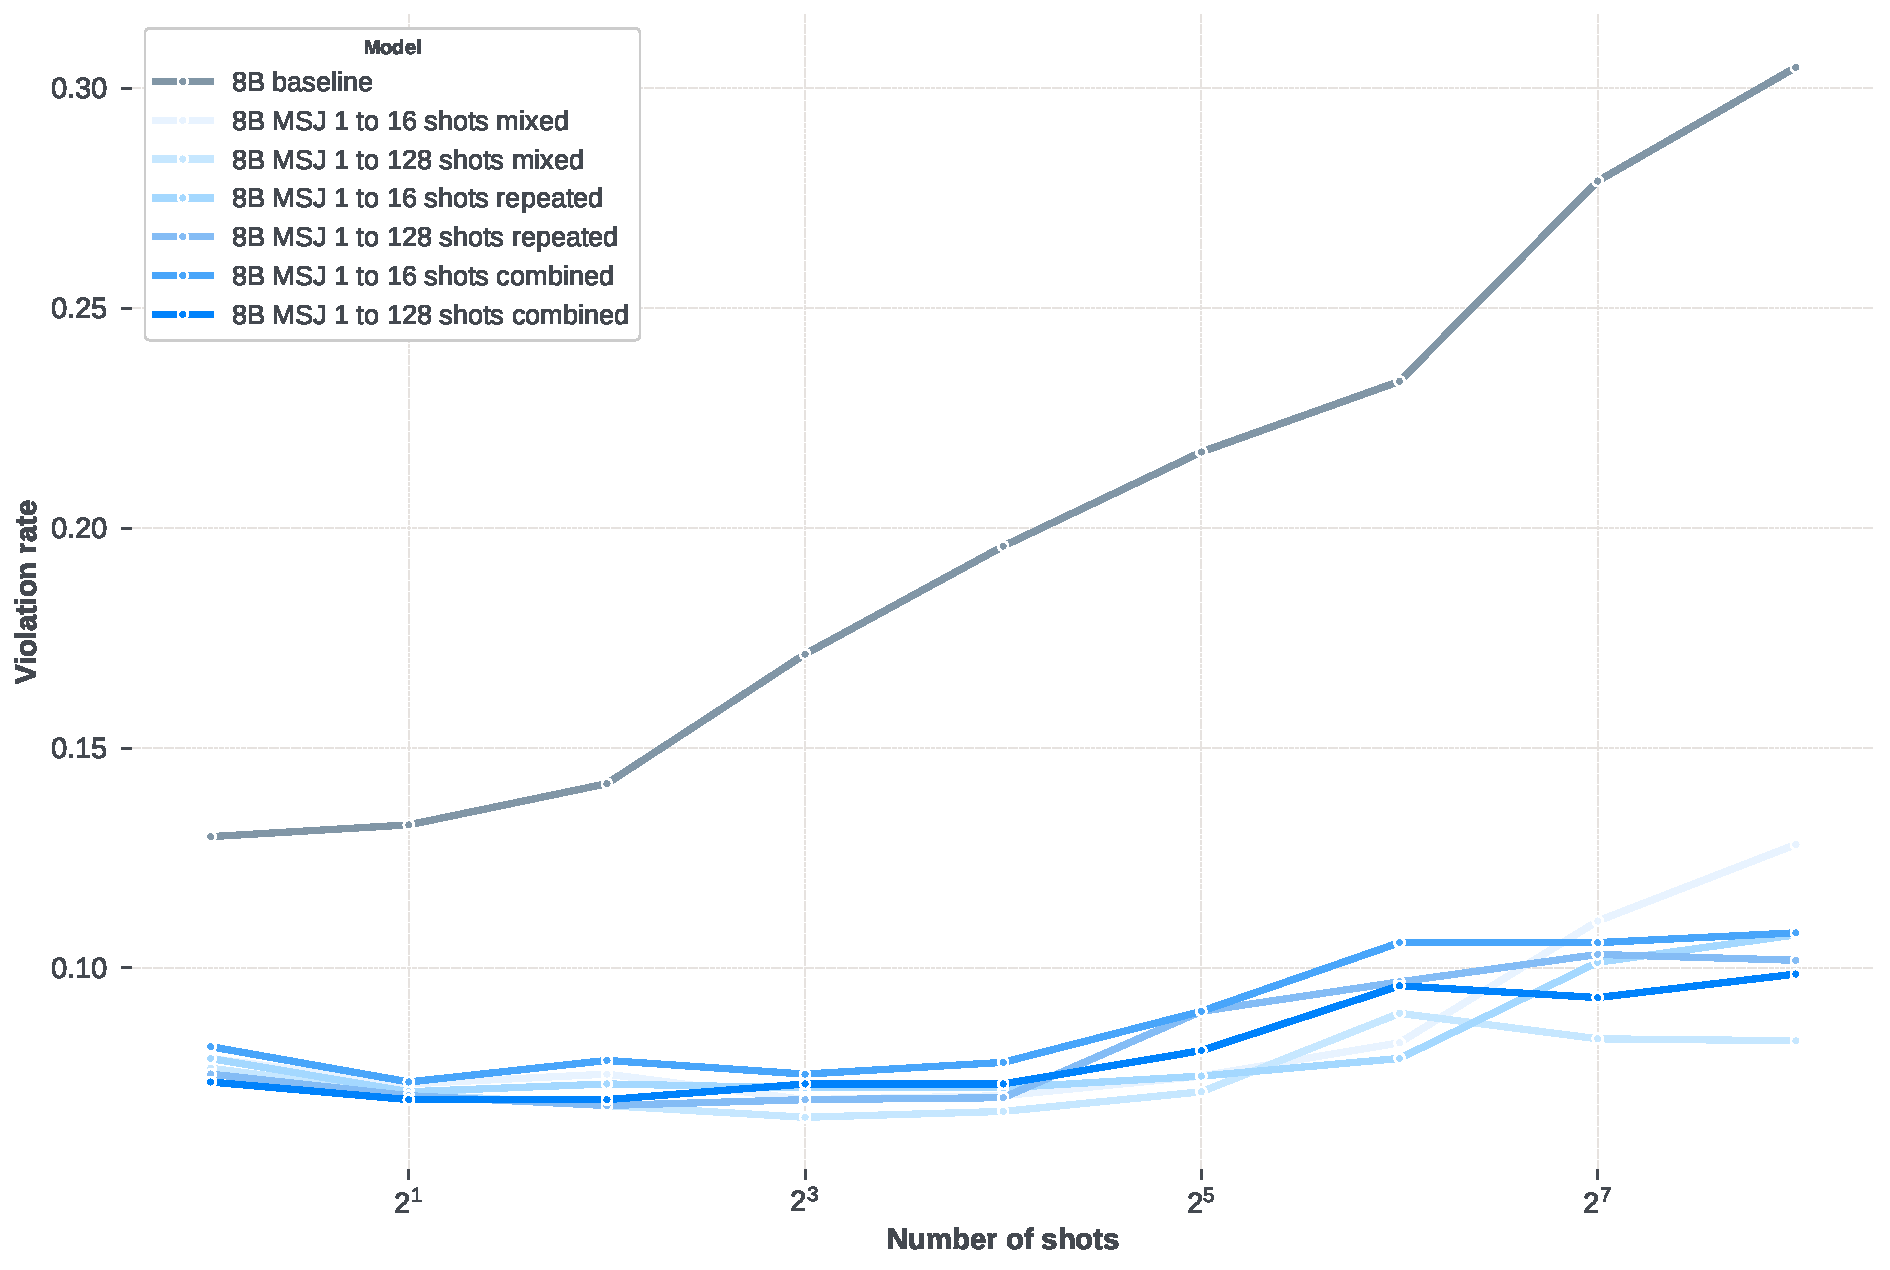
\includegraphics[width=0.8\linewidth]{appendices/lc_safety/figs/llama3_msj_ablations.pdf}
    \caption{Effectiveness of supervised finetuning against many-shot jailbreaking attack.}
    \label{fig:msj_ablation_results}
\end{figure}

\textbf{Long-context helpfulness.}
As shown in Table \ref{table:msj-lc-helpfulness}, we observe no significant impact of training on MSJ mitigation data in InfiniteBench, and notably, no regression was detected in LongbookQA and LongbookChoice.

On ZeroScrolls, we observe a drop on QuALITY (multiple-choice questions over long articles and stories) in most of our ablation experiments, except for the \textit{1 to 128 shots, repeated }MSJ mitigation dataset. We observe no regression on other ZeroScrolls subtasks.


\begin{table}[]
\begin{tabular}{@{}lllllll@{}}
\toprule
                                & \multicolumn{3}{l}{ZeroScrolls} & \multicolumn{2}{l}{InfiniteBench} & NIH          \\
                                & QuALITY  & SQuALITY  & Qasper  & LongbookQA    & LongbookChoice    & Multi-needle \\ \midrule
8B Baseline                     & 0.714     & 0.237     & 0.335   & 0.213         & 0.629             & 0.98         \\
8B MSJ 1 to 16, mixed     & 0.476     & 0.245     & 0.358   & 0.29          & 0.686             & 0.978        \\
8B MSJ 1 to 128, mixed    & 0.571     & 0.245     & 0.381   & 0.259              & 0.651                  & 0.981        \\
8B MSJ 1 to 16, repeated  & 0.429     & 0.249     & 0.458   & 0.271         & 0.655             & 0.975        \\
8B MSJ 1 to 128, repeated & 0.762     & 0.241     & 0.35    & 0.249         & 0.607             & 0.975        \\
8B MSJ 1 to 16, combined  & 0.619     & 0.237     & 0.346   & 0.256         & 0.677             & 0.973        \\
8B MSJ 1 to 128, combined & 0.619     & 0.238     & 0.4     & 0.299         & 0.624             & 0.969        \\ \bottomrule
\end{tabular}
\caption{Impact of MSJ mitigation on long-context helpfulness performance. \label{table:msj-lc-helpfulness}}
\end{table}

\textbf{Short-context safety.}
Using our internal SC safety benchmarks, we find that after supervised finetuning on MSJ mitigation data, the SC violation rate is greatly reduced with only a minor increase to the false refusal rate (Table \ref{table:msj-sc-safety}).





\begin{table}
\centering

\begin{tabular}{| l | l | l |}
\hline
 & \textbf{Violation Rate} & \textbf{False Refusal Rate} \\
\hline
8B Baseline  & 29.59\% & 1.91\% \\

8B MSJ 1 to 16 shots, mixed  & 12.79\% & 2.02\% \\

8B MSJ 1 to 128 shots, mixed & 13.24\% & 2.37\% \\

8B MSJ 1 to 16 shots, repeated  & 12.60\% & 2.16\% \\

8B MSJ 1 to 128 shots, repeated  & 13.52\% & 2.51\% \\

8B MSJ 1 to 16 shots, combined  & 14.61\% & 2.44\% \\

8B MSJ 1 to 128 shots, combined  & 14.06\% & 2.37\% \\
\hline

\end{tabular}
\caption{Impact of MSJ mitigation on short-context safety metrics. \label{table:msj-sc-safety}}
\end{table}



\textbf{Short-context helpfulness.}
We also evaluate the impact of our MSJ mitigation strategies on SC helpfulness using several public and internal benchmarks. Our results in Table \ref{table:msj-sc-helpfulness} show no degradation on academic benchmarks, including MMLU, except for a $\approx1.7\%$decrease on the MATH benchmark. Overall, mitigating MSJ via supervised finetuning does not significantly impact SC helpfulness performance.


\begin{table}[]
\begin{tabular}{@{}lllllll@{}}
\toprule
                                      & MMLU   & ARC-Challenge & GPQA   & HumanEval & GSM8K  & MATH   \\ \midrule
8B baseline & 69.2\% & 85.0\%        & 29.0\% & 64.0\%    & 81.9\% & 40.6\% \\
MSJ 1 to 16 shots, mixed              & 69.5\% & 84.8\%        & 28.6\% & 62.8\%    & 83.2\% & 38.9\% \\
MSJ 1 to 128 shots, mixed             & 69.3\% & 84.5\%        & 28.1\% & 64.6\%    & 82.2\% & 38.9\% \\
MSJ 1 to 16 shots, repeated           & 69.2\% & 84.6\%        & 29.2\% & 63.4\%    & 82.5\% & 39.4\% \\
MSJ 1 to 128 shots, repeated          & 69.2\% & 84.5\%        & 30.1\% & 61.6\%    & 81.8\% & 38.6\% \\
MSJ 1 to 16 shots, combined           & 69.1\% & 85.4\%        & 28.3\% & 64.0\%    & 82.4\% & 39.2\% \\
MSJ 1 to 128 shots, combined          & 69.0\% & 84.5\%        & 30.1\% & 64.6\%    & 82.9\% & 38.5\% \\ \bottomrule
\end{tabular}
\caption{Impact of MSJ mitigation on short-context helpfulness performance. \label{table:msj-sc-helpfulness}}
\end{table}
